\documentclass[times, utf8, seminar]{fit}

%\batchmode
%\usepackage{booktabs}
\usepackage{listings}
\usepackage{longtable}
\usepackage{xcolor}
\usepackage{float}
\usepackage{enumitem}
\usepackage{hyperref}

\begin{document}

\title{Poslovna inteligencija bazirana na "open source" softveru}

\author{Ernad Husremović}
\brindex{DL 2792}
\verzija {2.0.2}

\mentor{prof.dr Vanja Bevanda}

\maketitle

\tableofcontents

\chapter{Uvod}

\section{Poslovna inteligencija (BI)}

Poslovna inteligencija (nadalje BI\footnote{BI Business intelligence}) se primarno odnosi na računarski bazirane tehnike identificiranja, ekstrakcije i analize poslovnih podataka.  BI tehnologije obezbjeđuju pregled ranijih i tekućih poslovnih operacija, kao i predviđanje budućih trendova u poslovanju\footnote{prediktivna analiza} \cite{web:wikipedia:bi}.

Standardne funkcije BI-a su:

\begin{enumerate}
  \item izvještavanje (reporting)
  \item analitičko procesiranje (analitycal processing)
  \item rudaranje podataka (data mining)
  \item prediktivne analize (predictive analytics)
\end{enumerate}

Sve ove funkcije pomažu poslovnom odlučivanju i planiranju - kako strateškom\footnote{Odlučivanje `top' managera} tako i operativnom planiranju\footnote{`department' manageri}.

\subsection{Operativni podaci, skladišta podataka}
\label{operativni_podaci}

BI kao izvor podataka koristi skladišta podataka.

Skladišta podataka treba razlikovati od operativnih podataka. Operativni podaci - podaci o tekućem poslovanju nalaze se unutar poslovnih aplikacija (ERP)\footnote{ERP - Enterprise Resource Planning software, software za podršku tekućem poslovanju}.

ERP sistemi pohranjuju poslovne transakcije (poslovne dokumente) u realnom vremenu.

ERP sistemi sadrže sisteme izvještavanja\footnote{ Tradicionalni reporting sistem. Podjelu na tradicionalni i BI reporting treba ipak uslovno postaviti. Mnogi savremeni ERP sistemi imaju u svom sastavu segmente BI reporting-a} koji su prevashodno usmjereni na davanje (detaljnih) podataka o tekućem poslovanju\footnote{period tekuće poslovne godine do nivoa pojedinačne poslovne transakcije}. 
 
Operativni podaci su glavni izvor za gradnju skladišta podataka. Međutim, skladišta podataka se najčešće grade iz heterogenih izvora.

Iako slični po načinu konstrukcije, u BI terminologije se pravi distinkcija  između `data mart' i `data warehouse' skladišta podataka\footnote{U domaćoj literaturi se najčešće za oba pojma koristi termin `skladište podataka'}:  

\begin{description}
  \item [Data mart (DMart)] sadrži informacije o jednom dijelu organizacije (npr. prodaja, ljudski resursi),
  \item [Data warehouse (DW)] sadrži informacije iz više područja - analizira organizaciju globalno.
\end{description}
 
DW je stoga usmjeren na podršku 'top' menadžmenta, dok DMart obezbjeđuje informacije za upravljanje i operativno planiranje pojedinih dijelova organizacije \cite[str.~391]{pentaho32}.

\section{Poslovni motivi za implementaciju BI rješenja}

Analiza poslovnih podataka u cilju podrške kvalitetnom poslovnom odlučivanju postojala je informatizacije poslovanja.

Slijedeća poslovna pitanja su univerzalna (nisu aktuelna tek u informatičkoj eri):

\begin{itemize}
  \item Kako se kretala prodaja određene grupe artikala u predhodnom periodu ?
  \item Koja grupa artikala se najviše zadržava na lageru ?
  \item Kakva je struktura prodaje po regijama ?
  \item Unutar koje grupacije artikala / proizvoda je najbolja marža ?
\end{itemize} 

Sva ova pitanja praktično vrše analizu efekata poslovanja usljed različitih uticaja (multidimenzionalna analiza).

Iz svih gornjih pitanja mogu se uočiti dva tipa informacija:

\begin{itemize}
   \item mjere - poslovni indikatori (prodaja, vrijednost zalihe, visina marže)
   \item dimenzije - atributi poslovanja (geografske dimenzije - grad, region, vemenske dimenzije, grupe artikala, rang cijena ...)
\end{itemize}

Ovaj koncept je polazište za konstrukciju multidimenzionalnih skladišta podataka (OLAP cube) kao osnovnog gradivnog elamenta BI rješenja.
 
\subsection{OLAP kocka}

OLAP kocka  (OLAP cube\footnote{OLAP - online analytical processing}) je set podatka organizovanih na taj način da omogućavaju \emph{nedeterminirane} upite nad agregiranim podacima, odnosno online analitičko procesiranje podataka \cite{web:wikipedia:olap_cube}.

Ovakva organizacija podataka omogućava OLAP klijentima pregled podataka u različitim varijantama.

Ono što RDBMS\footnote{RDBMS relational database management system} predstavlja za ERP sistem, OLAP kocka predstavlja za BI sistem.

Analogija postoji i u dijelu pretrage podataka:

\begin{itemize}
 \item RDBMS <-> SQL structured query language
 \item OLAP cube <-> MDX - multidimensional query language
\end{itemize}

Današnje implementacije OLAP kocki su slijedeće:

\begin{itemize}
  \item ROLAP - podaci smješteni u relacijske baze podataka
  \item MOLAP - podaci su u proprietary formatu prilagođenom procesiranju multidimenzionalnih struktura podataka
\end{itemize}

Pored gornjih postoje i hibridne implementacije OLAP kocki koje kombinuju gornje tehnologije.

\subsection{Alati za integraciju podataka (DI)}

DI\footnote{DI - data integration} alati mogućavaju vezu BI sistema sa "vanjskim" svijetom (vidi \ref{operativni_podaci} operativni podaci)

Glavni dio DI `toolset'-a su je ETL softver\footnote{ETL - Extract/Transform/Load}. 

ETL softver obavlja sljedeće funkcije:

\begin{enumerate}
  \item \emph{Extract:}  uzimanje podataka iz vanjskih izvora
  \item \emph{Transform:} transformacija operativnih podataka u format koji je pogodan za pohranu u skladište podataka (vidi \ref{operativni_podaci})
  \item \emph{Load:} snimanje `prečišćenih' podataka u skladište podataka (DW/DMart)
\end{enumerate}
 
\subsection{Rudarenje podataka (DM)}

Pojam rudaranje podataka\footnote{DM - data mining} se može definisati kao pronalaženje zakonitosti među podacima. 

Jedna od definicija rudaranje glasi: rudarenje podataka je sistematičan, interaktivan i iterativan proces izvođenja i prikazivanja korisnika, implicitnog i inovativnog \emph{znanja} iz podataka \cite[str.~40]{mag_mrsic}.

Unutar ovog rada nećemo se baviti ovim dijelom BI-a.

\subsubsection {Dodatno proučavanje}

Open source software koji pokriva ove oblasti:
 
\begin{itemize}
  \item Data mining `Weka' projekat: \cite{web:weka}, \cite{web:pentaho_weka}
  \item `R' statistički paket \cite{web:r} - prediktivne, trend analize
\end{itemize}

Treba uočiti da je `Weka' jedan od podprojekata `Pentaho BI suite'-a (vidi \ref{sect:pentaho}).

\chapter{"Open source" (OSS) BI software}

"Open source" (nadalje OSS\footnote{OSS - open source software}) rješenja dostupne su za sve glavne funkcije BI-a.
 
Najveći OSS BI projekti vođeni su od strane komercijalnih opensource vendora. Najpoznatiji OSS BI vendori su:

\begin{itemize}
 \item Jaspersoft BI \footnote{\url{http://www.jaspersoft.com/}}
 \item Pentaho BI \footnote{\url{http://www.pentaho.com/}}
 \item Talend\footnote{\url{http://www.talend.com/}}
\end{itemize}
 
Treba naglasiti da su mnoge komponente pojedinih BI rješenja bazirane na istim tehnologijama ili su čak identične.

Tako vendori koji su na komercijalnom polju konkurencija, zajednički rade na razvoju baznih komponenti. 

Ova sinergija u razvoju, što je uostalom generalna odlika OSS-a, predstavlja snažan poticaj brzom razvoju OSS BI rješenja.

\section{"Open core" model}

Većina opensource BI vendora bazira se na `open core' modelu. Ovaj model organizacije opensource softvera predviđa dvije verzije:
\begin{itemize}
  \item "community" verzija (OSS),
  \item "enterprise" verzija (`closed source', `proprietary addon'-ovi vendora)
\end{itemize}

\section{Pentaho BI}

Pentaho BI obuhvata praktično funkcije BI-a \cite[str.~7]{pentaho32}:

\begin{enumerate}
 \item multidimenzionalna analiza
 \item izvještavanje
 \item BI "dashboards"\footnote{prikaz glavnih poslovnih indikatora u putem sažetog grafičkog prikaza}
\end{enumerate}

\begin{figure}[H]
\centering
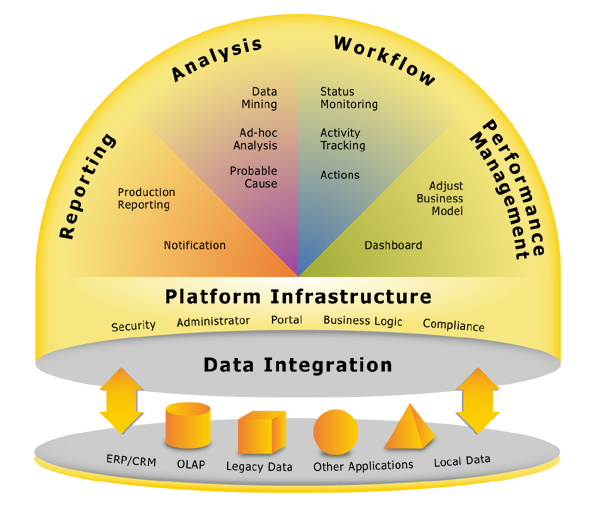
\includegraphics[width=12cm]{img/pentaho_arhitektura_eric.png}
\caption{Pentaho arhitektura (\cite{web:eric})}
\end{figure}

\section{Komponente Pentaho BI-a}
\label{sect:pentaho}

\subsection{Mondrian OLAP}

Pentaho implementacija OLAP kocke naziva se `Mondrian'. Mondrian je kocka ROLAP tipa.

Treba pomenuti da je `Mondrian'  XMLA kompatibilan provajder\footnote{XML za Analizu (XMLA) je industrijski standard za pristup podacima u analitičkim sistemima kao što su OLAP i `data mining'. Baziran je na drugim industrijskim standardima kao što su XML, SOAP i HTML \cite{web:wikipedia:xmla}.}


\subsection{Mondrian OLAP shema}

Kao ROLAP implementacija, podaci se nalaze u relacijskog bazi podataka\footnote{Podržane su sve JDBC podržane relacijske baze: PostgreSQL, MySQL, MSSQL, Oracle}

Kod konstrukcije sheme koriste se sljedeći pojmovi:

\begin{itemize}
  \item `dimension table' - tabela u kojoj su pohranjene dimenzije
  \item SCD - slow changing dimension {\cite[poglavlje ~12]{pentaho32}}
  \item SCD Type I - čuva se samo jedna vrijednost dimenzije
  \item SCD Type II - čuva se istorija vrijednosti dimenzije kroz vremenski period \footnote{npr. cijena artikla se mijenja tokom vremena, SCD type II dimenzija za svaku novu cijenu pravi novi zapis u dimension tabeli}
  \item `facts table' - tabela u kojoj su mjere - poslovni indikatori koje analiziramo
  \item `business key' (bk) - ključ koji koriste aplikacije za rukovanje operativnim podacima (ERP software)
  \item `surogat key' (id) - ključ u bazi podataka koji koristi OLAP storage
  \item `snowflake' shema - šema u kojoj su dimenzije u sopstvenim tabelama, dimenzije su visokog stepena normalizacije podataka\footnote{normalizacija podataka u relacijskog bazi podataka} \cite{web:pentaho:mondrian_schema}
  \item Type II
\end{itemize}

Pogledajmo jednu gotovu mondrian shemu dobijenu u \emph{case study}-ju (pogl. \ref{chap:case_study}) koji slijedi:

\begin{figure}[H]
\centering
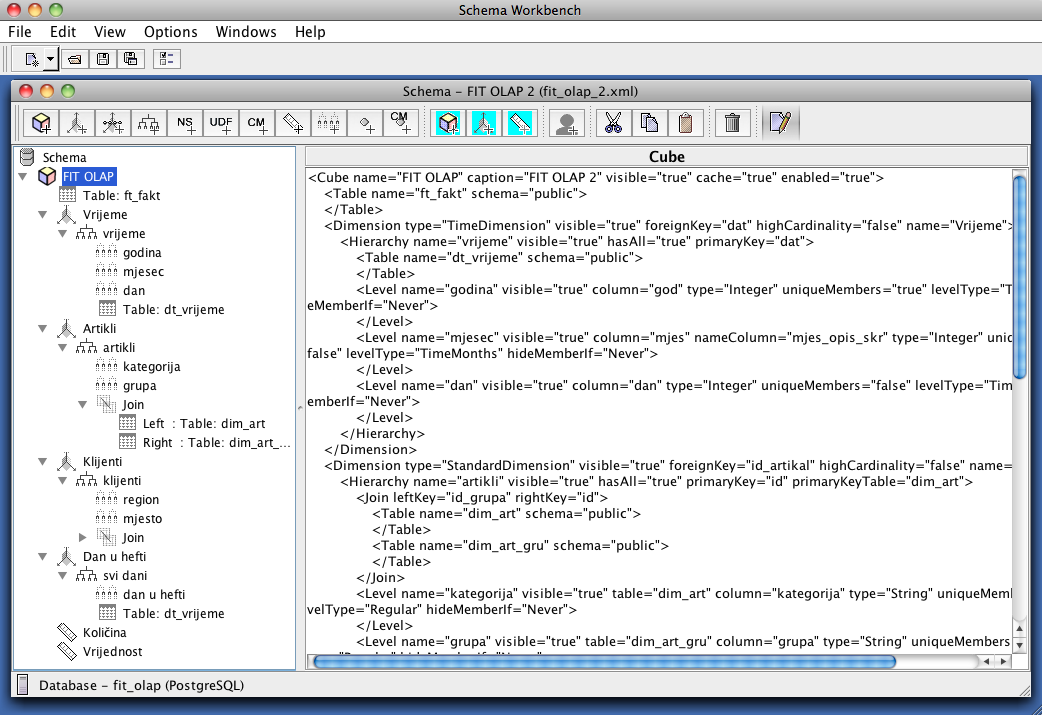
\includegraphics[width=15cm]{img/fit_olap_mondrian_schema.png}
\caption{Mondrian schema OLAP 2 cube}
\label{fig:mondrian_schema}
\end{figure}


\subsection{Pentaho ETL dizajner `Spoon'}

`Spoon' je GUI aplikacija u kjoj se vrši definicija i testiranje ETL transformacija i `job'-ova.

Kod ETL operacija bitno je poznavati sljedeće pojmove:

\begin{itemize}
  \item 'cleansing` - "čišćenje" podataka - ispravka (ili izbacivanje) netačnih podataka
\end{itemize}

\subsection{Analiziranje OLAP kocki}

Pentaho sadrži dva `OLAP analyzer'\footnote{često se za ove aplikacije kaže `OLAP cube client' ili 'OLAP data consumer' aplikacije} rješenja:

\begin{itemize}
  \item JPilot - starije rješenje, napušta se njegov razvoj\footnote{označeno od Pentaho razvojnog tima kao `deprecated'}
  \item novi `OLAP Analyzer' koji se nalazi samo u `Enterprise' (plaćenoj verziji)\footnote{kako je ova komponenta je `closed source' sofware, ona se u ovom radu neće razmatrati.}
\end{itemize}

Kao `OLAP Analysis' sofver izabran je Saiku (vidi \ref{chap:biljeske}).

Saiku je modularni `open source' analitički sotver koji nudi jednostavnu OLAP analizu podataka \cite{web:saiku}

Kod korištenja OLAP analitičkog softvera koriste se sljedeći pojmovi:

\begin{itemize}
  \item redovi - sadrži jednu ili više mjera i/ili dimenzija koje se prikazuju u redovima kod prikaza podataka
  \item kolona - sadrži jednu ili više mjera i/ili dimenzija koji se prikazuju u kolonama prikaza podatka
  \item filteri - ograničenje podataka po određenim vrijednostima dimenzija
\end{itemize}

\chapter{Case study: Kreiranje i analiza 'Mondrian' OLAP kocke}
\label{chap:case_study}

U ovom `case study'-ju ćemo izvršiti formiranje OLAP kocke za operativne podatke ERP aplikacije `F18 knowhow' radi analize podataka o prodaji.  

\section{F18 knowhow ERP}

\begin{figure}[H]
\centering
\includegraphics[width=15cm]{img/F18_erp.png}
\caption{ERP aplikacija, F18 klijent}
\end{figure}

\section{Poslovni cilj}

Cilj je analizirati prodaju firme firme "bring.out"\footnote{\url{http://www.bring.out.ba}} po godinama pri čemu nas interesuje struktura klijenata po gradovina i regionima, te prodaja artikala po određenim kategorijama i grupama.

Znači, potrebno je kreirati DMart prodaje za kompletan period poslovanja (1996-2011). 

Glavni operativni podaci nalaze se u ERP aplikaciji, u PostreSQL relacijskoj bazi. 

Dio potrebnih dimenzija (regioni, kategorije i grupe artikala) nisu implementirani unutar operativnih podataka, tako da analitičar mora unutar ETL procesa ove informacije dodati. 

Podaci svake poslovne godine nalaze se u posebnoj bazi podataka.

Operativni podaci `F18 knowhow' smješteni su u sljedeći relacijski model:

\begin{figure}[H]
\centering
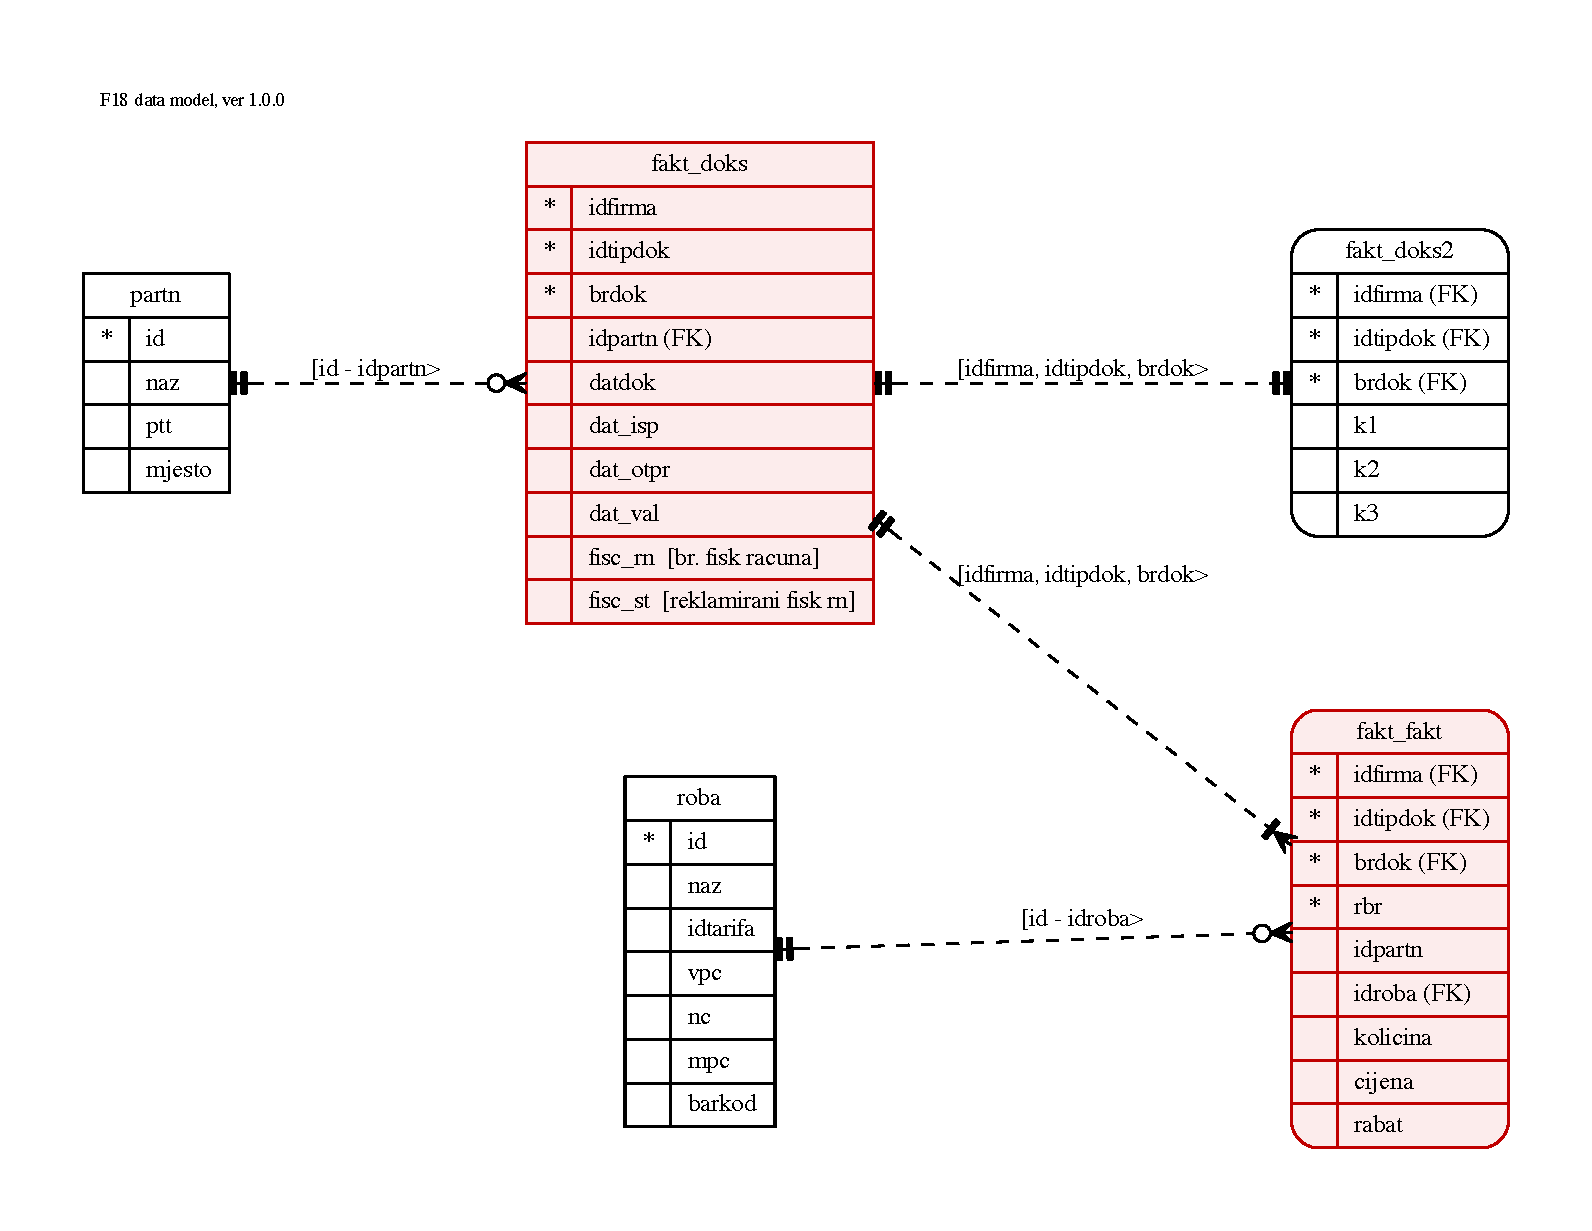
\includegraphics[width=15cm]{img/F18_db.pdf}
\caption{F18 transakcijski db model (relevantni dio)}
\end{figure}

\section{Model skladišta podataka (DMart)}

Na osnovu gornjeg zahtjeva utvrđujemo model skladišta podataka koji ćemo koristiti za igradnju OLAP kocke:

\begin{figure}[H]
\centering
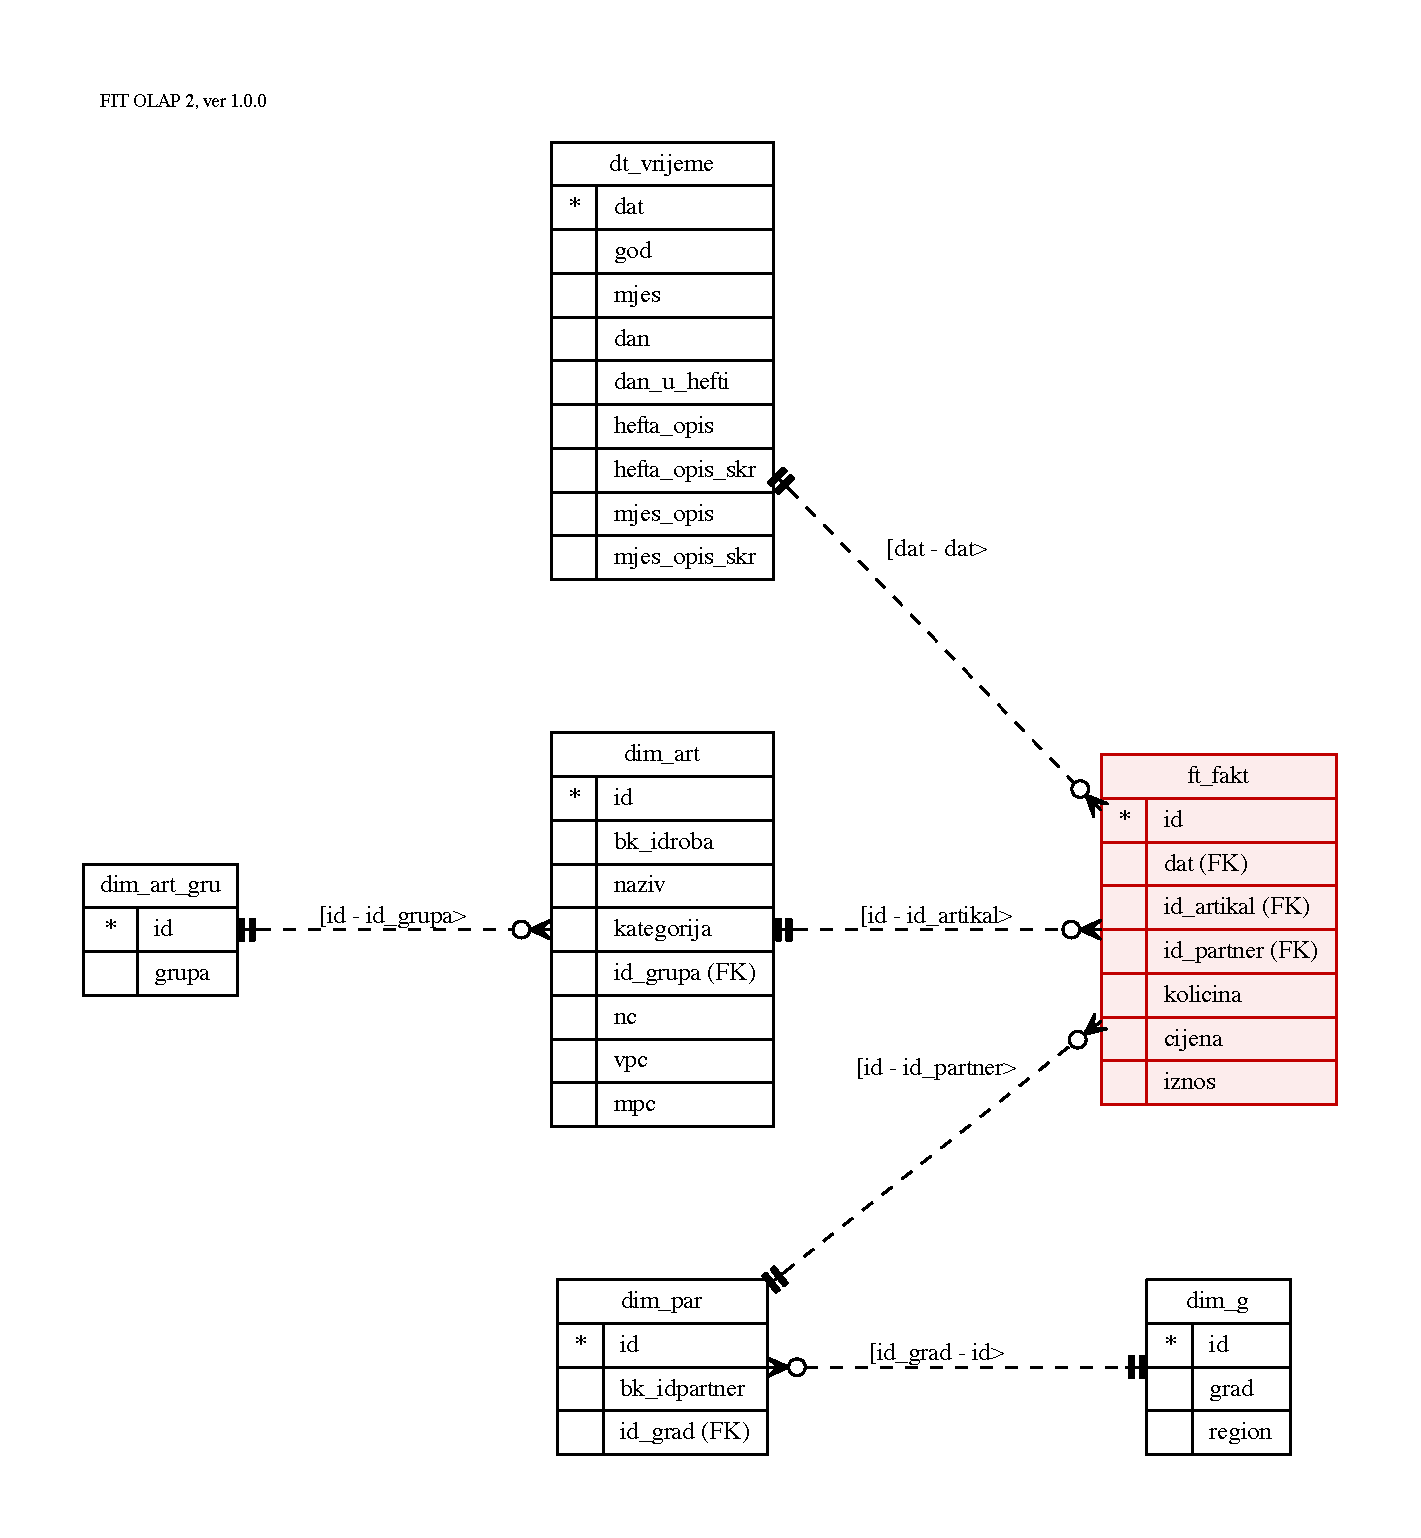
\includegraphics[width=15cm]{img/F18_olap.pdf}
\caption{OLAP schema}
\end{figure}


\section{Trasformacija operativnih podataka: klasifikacija i `cleansing'}

F18 `cleansing' podataka vrši se na šifarskom sistemu (matičnim podacima) artikala i klijenata.

Za te potrebe se u kettle transformacijama prlikom formiranja odgovarajućih dimenzija vrši `lookup' na osnovu posebno pripremljenih tabelarnih podataka (vidi \ref{chap:izvorni_kod}, olap\_cleansing xls dokument).

\subsection{Šifrarnik artikala}

\begin{figure}[H]
\centering
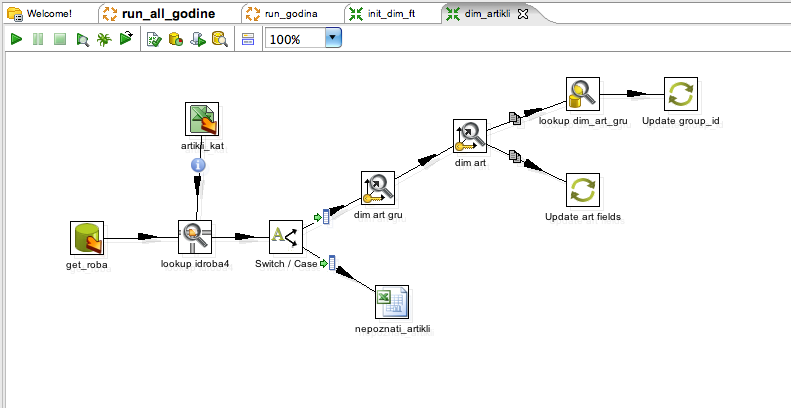
\includegraphics[width=15cm]{img/kettle_tr_dim_artikli.png}
\caption{Kettle transformacija: Generacija "dim\_art" i "dim\_art\_gru" `dimension' tabela za određenu poslovnu godinu}
\end{figure}

\begin{figure}[H]
\centering
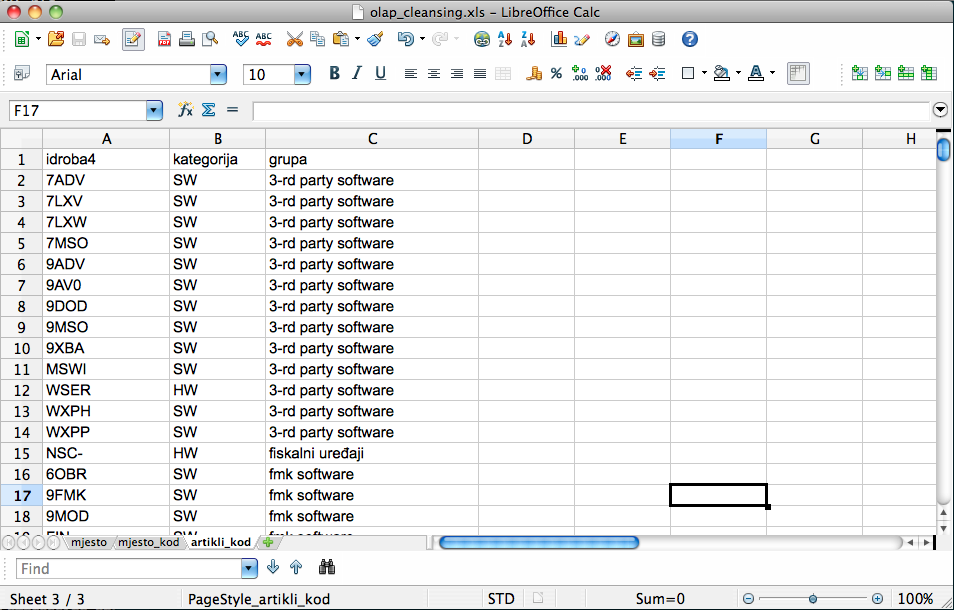
\includegraphics[width=15cm]{img/clean_artikli.png}
\caption{F18 klasificiranje - šifarski sistem artikala}
\end{figure}


\subsection{Šifrarnik klijenata}

\begin{figure}[H]
\centering
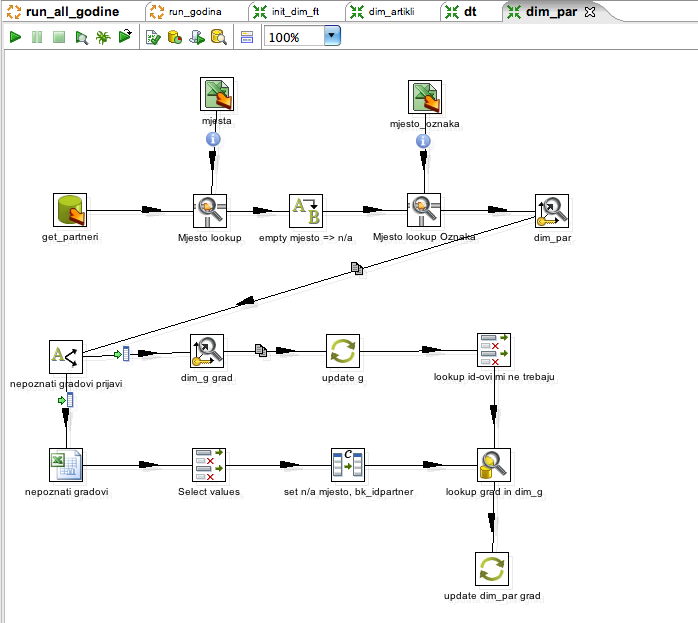
\includegraphics[width=15cm]{img/kettle_tr_dim_par.png}
\caption{Kettle transformacija: Generacija "dim\_par" i "dim\_g" `dimension' tabela za određenu poslovnu godinu}
\end{figure}


\begin{figure}[H]
\centering
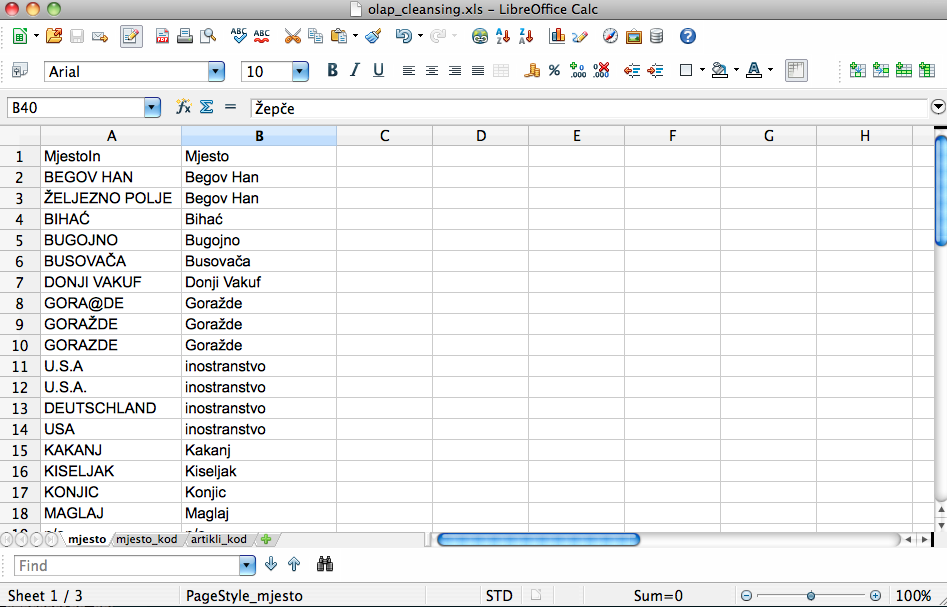
\includegraphics[width=15cm]{img/clean_mjesto.png}
\caption{`cleansing' F18 podataka -  klijenti - mjesta/gradovi}
\end{figure}


\begin{figure}[H]
\centering
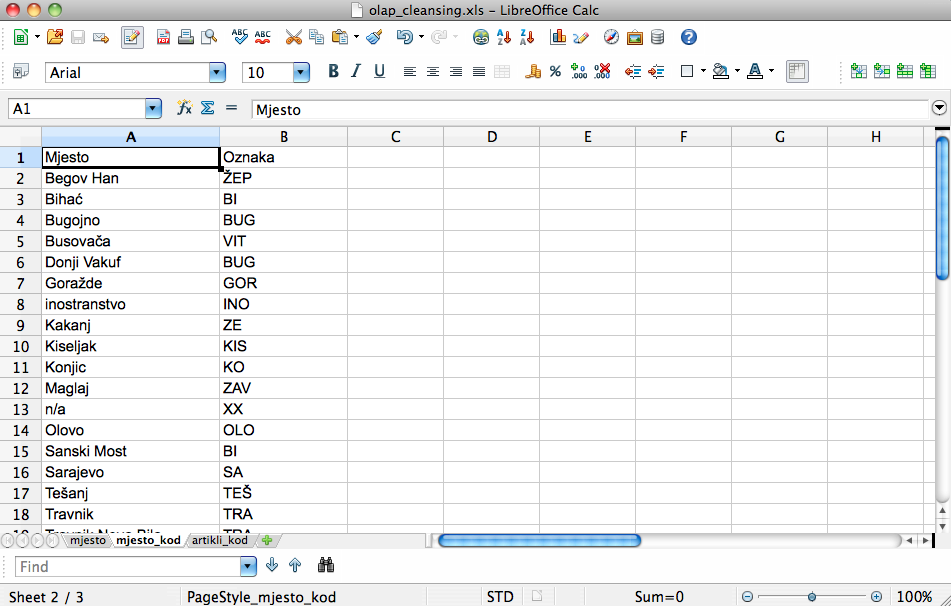
\includegraphics[width=15cm]{img/clean_mjesto_region.png}
\caption{F18 kodiranje regiona - klasifikacija mjesta/gradova}
\end{figure}

\section{Kreiranje vremenske dimenzije}

\begin{figure}[H]
\centering
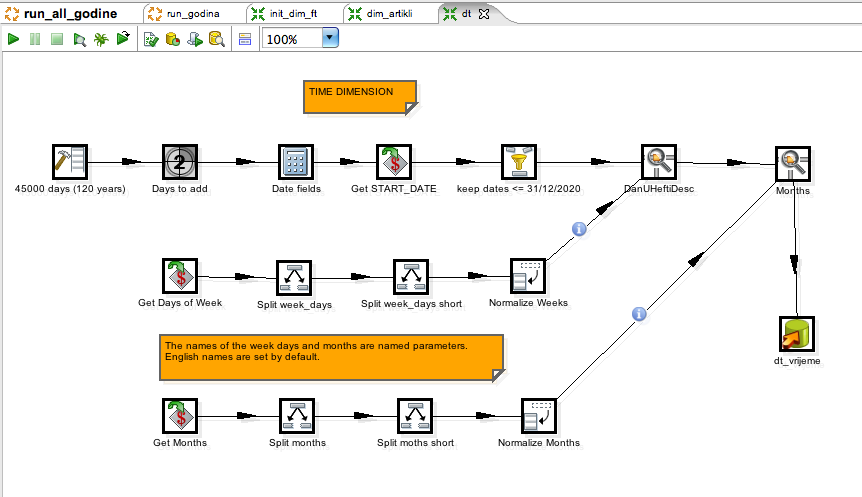
\includegraphics[width=15cm]{img/kettle_tr_dt.png}
\caption{Kettle transformacija: Generacija "dim\_dt" `dimension' tabele - vremenska dimenzija}
\end{figure}


\section{Kreiranje `facts' tabele prodaje}

\begin{figure}[H]
\centering
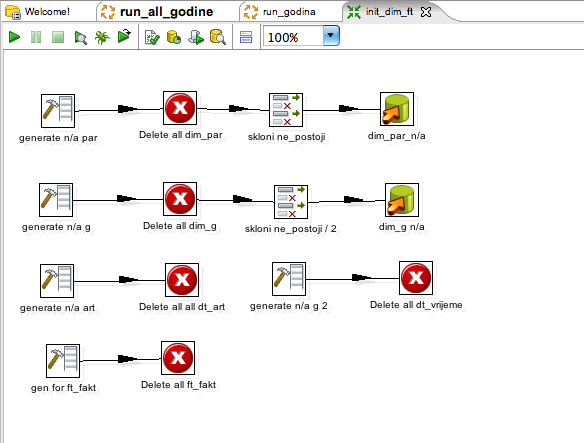
\includegraphics[width=15cm]{img/kettle_tr_init_dim_fpt.png}
\caption{Inicijalizacija `dimension' i `facts' tabela}
\end{figure}


\begin{figure}[H]
\centering
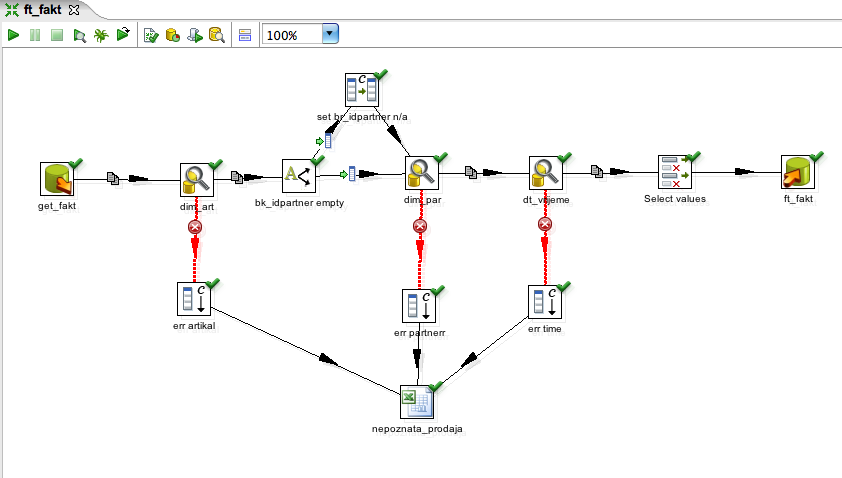
\includegraphics[width=15cm]{img/kettle_tr_ft_fakt.png}
\caption{Generacija "ft\_fakt" `facts' tabele za određenu poslovnu godinu}
\end{figure}

\section{Kettle `jobs'}

Kettle `job' omogućava nam da se pojedinačne transformacije i jednostavniji `job'-ovi integriraju u jedinstven ETL proces koji se može u automatizirati\footnote{kreiranje serverskih `batch' procesa}

\begin{figure}[H]
\centering
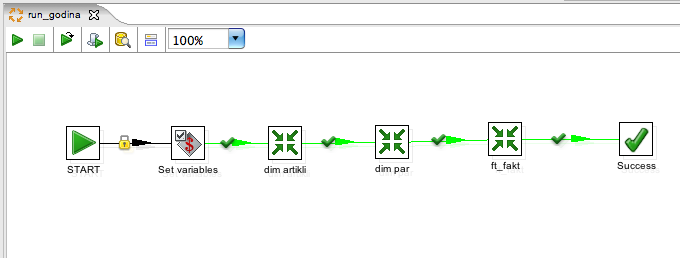
\includegraphics[width=15cm]{img/kettle_job_run_godina.png}
\caption{Kettle job: Generacija OLAP podataka iz F18 ERP izvora za jednu poslovnu godinu}
\end{figure}


\begin{figure}[H]
\centering
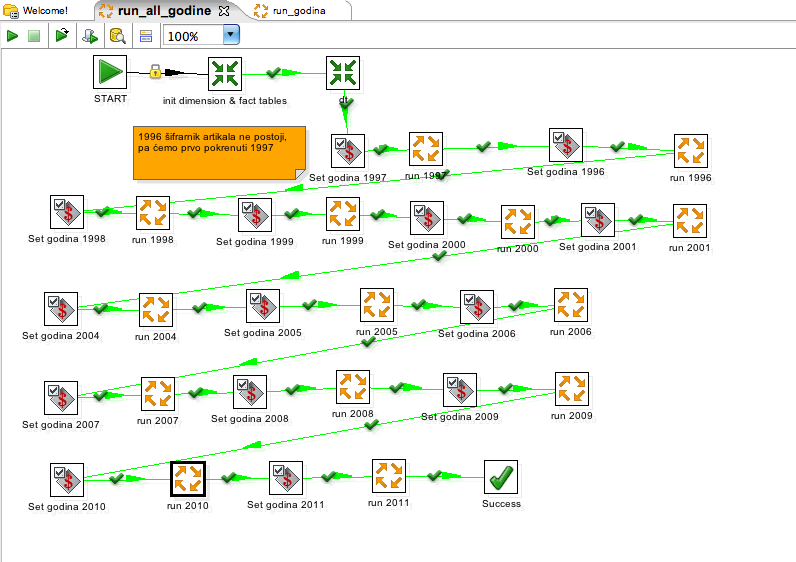
\includegraphics[width=15cm]{img/kettle_job_run_all.png}
\caption{Kettle job: inicijalizacija OLAP tabela, te generacija OLAP pdoataka za sve poslovne godine 1996-2011}
\end{figure}


\begin{figure}[H]
\centering
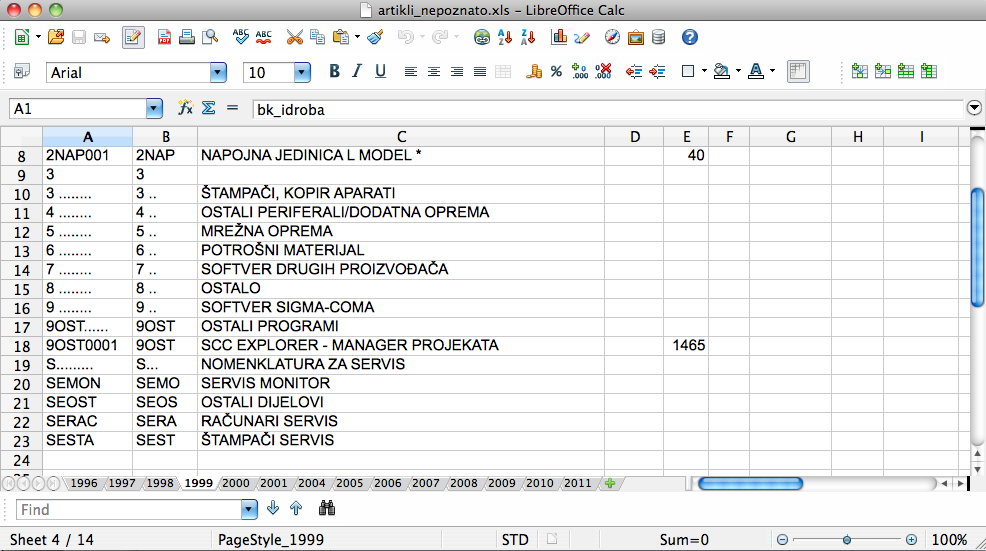
\includegraphics[width=15cm]{img/nepoznato_artikli.png}
\caption{Error reporting putem `spreadsheet' dokumenata - artikli za koje nisu definisani kodovi u olap\_cleansing tabelama}
\end{figure}

\begin{figure}[H]
\centering
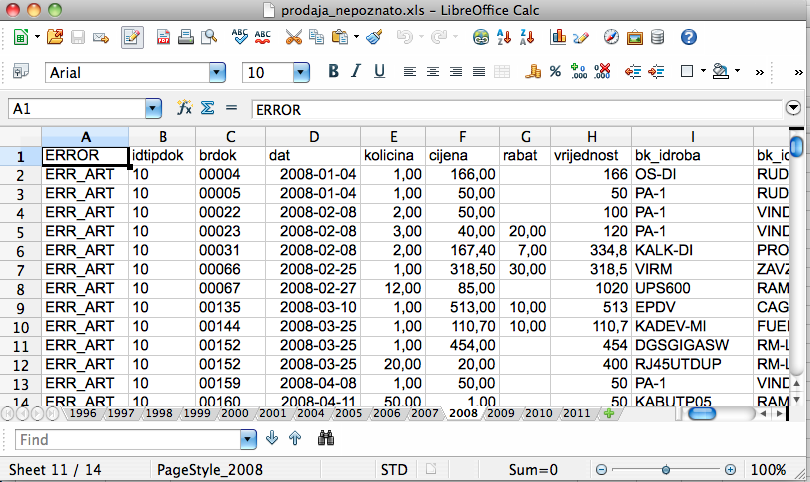
\includegraphics[width=15cm]{img/nepoznato_prodaja.png}
\caption{Dokumenti prodaje u kojima su neispravni podaci potrebni za popunjavanje dimension tabela (datum, klijent, roba) }
\end{figure}


\section{OLAP reporting} 

`Data mart' dobijen ETL procesom koristimo za podešavanje Mondrian sheme OLAP kocke (vidi sliku \ref{fig:mondrian_schema}). 

Dobijena shema se instalira na "Saiku" server. Saiku putem svog web interfejsa omogućava jednostavnu definiciju redova, kolona i filtera putem `drag \& drop' operacija.
   

\subsection{Pregled prodaje po grupama artikala}

\lstset{ %
   language=SQL,
   basicstyle=\small,
   numbers=left,
   numbersep=5pt,
   breaklines=true,
   backgroundcolor=\color{yellow!15},
   tabsize=2,
   keywordstyle=\color{blue},
   captionpos=b, 
   frame=none
}

\begin{figure}[H]
\centering
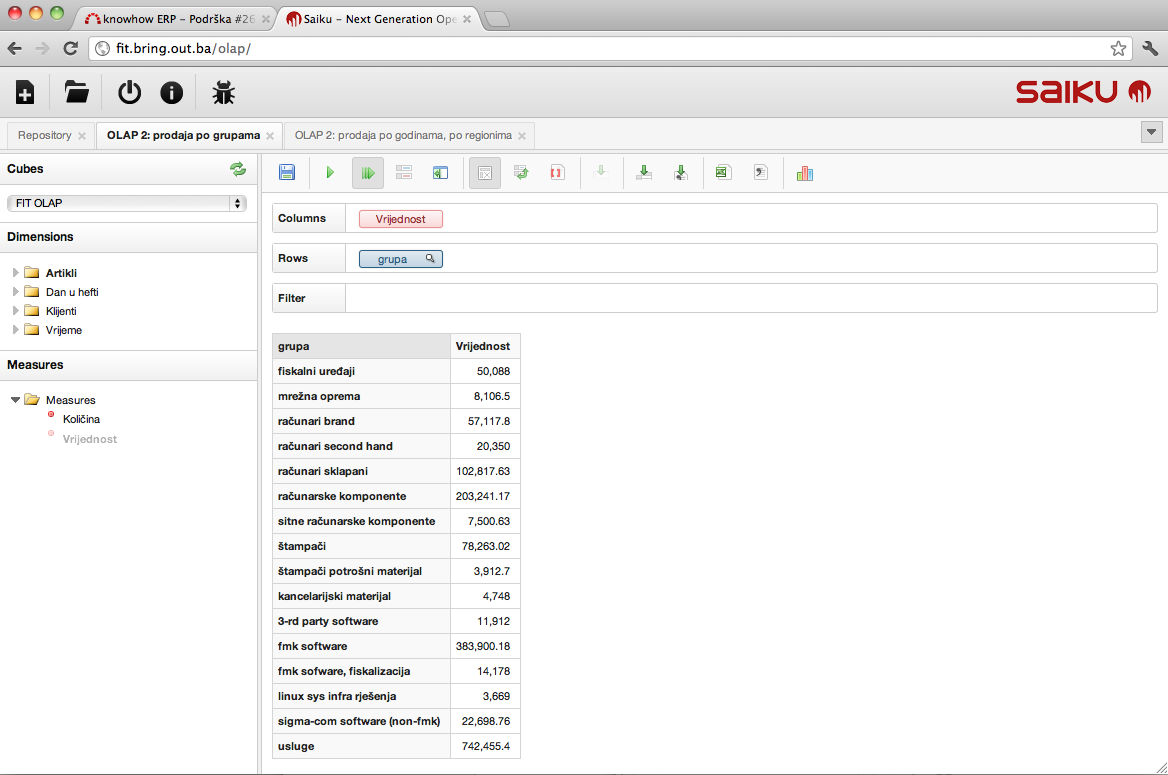
\includegraphics[width=15cm]{img/saiku_rpt_grupe}
\caption{Pregled prodaje po grupama artikala}
\end{figure}

`Saiku' automatski kreira `MDX query':

\lstset{caption={Pregled prodaje po grupama artikala}}
\begin{lstlisting}
SELECT
NON EMPTY {Hierarchize({[Measures].[Vrijednost]})} 
ON COLUMNS,
  NON EMPTY {Hierarchize({[Artikli.artikli].[grupa].Members})} 
ON ROWS
FROM [FIT OLAP]
WHERE {Hierarchize({[Vrijeme.vrijeme].[All Vrijeme.vrijemes]})}
\end{lstlisting}

\subsection{Pregled prodaje po regionima}

\begin{figure}[H]
\centering
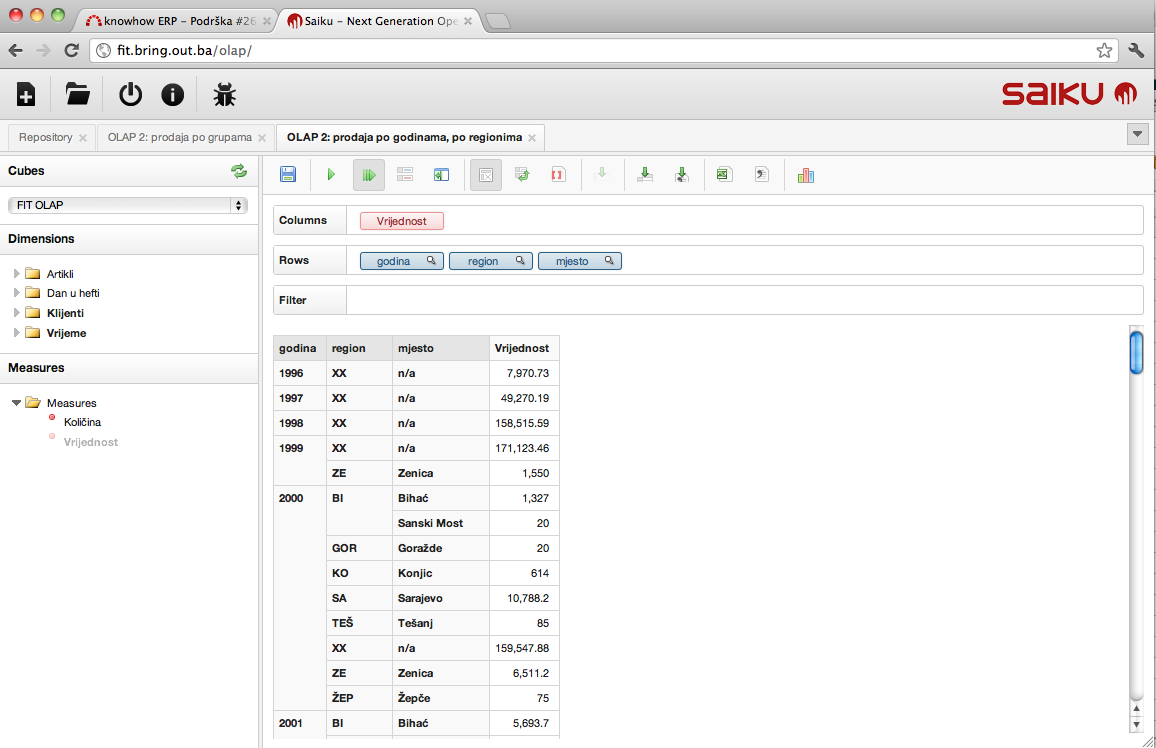
\includegraphics[width=15cm]{img/saiku_rpt_region}
\caption{Pregled prodaje po regionima, po godinama}
\end{figure}

\lstset{caption={Pregled prodaje po regionima}}
\begin{lstlisting}
SELECT
  NON EMPTY {Hierarchize({[Measures].[Vrijednost]})} 
ON COLUMNS,
  NON EMPTY 
    Hierarchize(
      Union(CrossJoin([Vrijeme.vrijeme].[godina].Members, 
      [Klijenti.klijenti].[region].Members), CrossJoin([Vrijeme.vrijeme].[godina].Members, 
      [Klijenti.klijenti].[mjesto].Members))
    ) 
ON ROWS
FROM [FIT OLAP]
\end{lstlisting}

Na gornjem izvještaju se mogu očiti mjesta sa oznakom 'n/a'. Naime, radi se o tome da se `cleansing' procesom nisu identificirali klijenti kod dijela poslovnih transakcija. Ti klijenti su označeni sa "n/a"\footnote{n/a - not available}.

Visoki iznosi za određene godine (1996-1999) indiciraju da postoje određeni propusti u ETL procesima za te podatke. 

Uzroke treba tražiti u ETL transformacijama vezanim za klijente. 

Detalji o neuspješnim transformacijama nalaze se u "nepoznato\_" spreadsheet dokumentima\footnote{primjer takvog dokumenta: dodatak \ref{chap:izvorni_kod}, artikli\_nepoznato xls dokument}. 

Vjerovatno je dovoljno kodirati nedostajuće šifre klijenata iz tih godina, te ponoviti kettle job proces "run\_all\_godine".

\chapter{Zaključak}

\section{Rezultati `case study'-ja}

Realizacijom `case study'-ja dobili smo `data mart' osnovnih parametara prodaje sa kojim smo konstruisali jednostavnu OLAP kocku.

Očekivano, najveći dio posla desio se u fazi pripreme podataka (ETL transformacije i `job'-ovi).

Analitičar mora dobro poznavati kako poslovnu domenu tako i tehnološke principe konstrukcije OLAP-a.

Ovakve poslove redovno rade timovi koji se sastoje od biznis analitičara i IT analitičara.

Da bi se došlo do iskoristivih podataka u skladištu podataka potrebna je velika uključenost klijenata (korisnika i vlasnika poslovnih procesa i podataka). 

Realni podaci sadrže puno netačnih ili nedostajućih podataka. U procesu sklapanja DW/DMart-a mnogi nedostaci mogu se otkloniti samo na osnovu dodatnih tumačenja podataka od strane klijenata. 

\section{Pogled sa aspekta menadžera}

S obzirom da sam kao kreator OLAP kocke ujedno i direktor firme čiji su podaci analizirani, iznijeću i par direktnih ddojmova kao klijent dobijene OLAP kocke:

\begin{itemize}
 \item Podaci o prodaji potvrđuju niz zaključaka do kojih sam kao nosilac poslovnih procesa dolazio "ad-hoc" zaključivanjem  
 \item Čak i ova jednostavna OLAP kocka omogućava mi da se fokusiram na određene aspekte poslovanja koje tradicionalnim reportingom nisam mogao postići
 \item Postojeća instalacija ukazala mi je na potrebu i mogućnosti koje bi dobio ovođenjem dodatnih indikatora poslovanja:
 \begin{itemize}
   \item uvođenje mjere broj\_radnika, te na osnovu toga omjer broj\_radnika / vrijednost\_realizacije po mjesecima, radi analize dosadašnjih efekata zapošljavanja
   \item finansijski troškovi po mjesecima
   \item trgovačka marža po mjesecima
 \end{itemize} 
\end{itemize}

Gornja zapažanja upućuju na naredne korake izgradnje skladišta podataka. Očigledno je da naš "data mart" prodaje treba dopuniti podacima iz drugih segmenata poslovanja (finansije, ljudski resursi). 

U ishodu, evolucija našeg BI rješenja vodi ka izgradnji "data warehouse"-a firme.

\section{Pogled sa aspekta informatičara}

Pentaho DI (kettle ETL) aplikacije imaju primjenljivost i van užeg konteksta izgradnje BI rješenja.

Oni su moćan alati u svim poslovima transformacije podataka. Mogu se koristiti za jednostavni "ad-hoc" reporting određenih podataka koje postojeći ERP sistem ne obezbjeđuje.

Njihov stepen integracije sa `spreadsheet' xls dokumentima daje mnoge mogućnosti koje su do sada isključivo tretirani oslovima koje samo software developeri mogu rješavati.

Ukratko, ovi alati značajno pomjeraju granice rukovanja i manipulacije poslovnih podataka.

\section{Rezime}

Izgradnja BI rješenja, čak i najjednostavnijeg koje je u `case study'-ju demonstrirano, traži značajne tehničke i poslovne resurse. 

Izgradnja BI rješenja je dugotrajan i skup proces koji sebi ne može priuštiti svaka organizacija. 

OSS BI rješenja tu granicu ipak mogu značajno pomjeriti u korist organizacija sa manjim budžetima.

\bibliography{literatura}
\bibliographystyle{fit}

\appendix

\chapter{Izvorni kod, dostupni resursi}
\label{chap:izvorni_kod}

\begin{enumerate}[labelindent=\parindent,leftmargin=*]
   \item OLAP mondrian, kettle transformacije i job-ovi, erviz modeli: \url{https://github.com/hernad/hello_bi}
   \item Latex kod ovog dokumenta \url{https://github.com/hernad/MIS/tree/master/latex}
   \item olap\_cleansing `spreadsheet' dokument \url{https://github.com/hernad/hello_bi/raw/master/olap_cleansing.xls}
   \item artikli\_nepoznato `spreadsheet' dokument \url{https://github.com/hernad/hello_bi/raw/master/artikli_nepoznato.xls}
   \item Saiku demo server online: \url{http://fit.bring.out.ba/olap/#}
\end{enumerate}

\chapter{Bilješke}
\label{chap:biljeske}

\begin{enumerate}
  \item Prva verzija ovog seminarskog rada, neuspješno \url{https://github.com/hernad/MIS/raw/master/knowhowERP_OLAP_blog_style.pdf}
  \item FIT OLAP 2 cube: \url{http://redmine.bring.out.ba/issues/26711}
\end{enumerate}

\end{document}
